\section{Fuzzy clustering}
%La clusterizzazione fuzzy, nota anche come soft k-means, è una tecnica avanzata di analisi dei dati che consente ai punti dati di appartenere a più di un cluster. Questa modalità differisce dalla tradizionale clusterizzazione "hard", dove ogni punto dati è assegnato esclusivamente a un singolo cluster, utilizzando invece una logica fuzzy per determinare l'appartenenza di un dato a ciascun cluster. In altre parole, anziché avere un'affermazione binaria di appartenenza (1 o 0), si ha una misura continua di appartenenza che varia da 0 a 1. Questo è espresso attraverso una funzione di similarità, $\mu_x(C)$, che rappresenta il grado di appartenenza di un dato $x$ a un cluster $C$.
Fuzzy clustering, also known as soft k-means, is a data analysis technique that allows data points to be assigned to more than one cluster. Unlike traditional "hard" clustering, where each data point is assigned exclusively to a single cluster, fuzzy clustering employs fuzzy logic to determine the degree of membership for each data point within multiple clusters. Instead of a binary membership statement ($1$ or $0$), fuzzy clustering provides a continuous measure of membership that ranges from $0$ to $1$. This is represented by a similarity function, $\mu_x(C)$, which quantifies the degree to which a data point $x$ belongs to a cluster $C$.

% referenza K-Means
%La clusterizzazione fuzzy ha le sue radici nel lavoro di J.C. Dunn, che nel 1973 ha introdotto questo concetto come un'estensione dell'algoritmo di clustering k-means. Dunn ha evidenziato la maggiore precisione e robustezza della clusterizzazione fuzzy rispetto alla clusterizzazione rigida, soprattutto nella gestione dei dati anomali (outlier) \citep{FuzzyClustering_developDoc}.
\noindent Fuzzy clustering originated from the work of \citeauthor{FuzzyClustering_developDoc}, who introduced this concept as an extension of the $k$-means clustering algorithm in $1973$. \citeauthor{FuzzyClustering_developDoc} emphasized the increased accuracy and robustness of fuzzy clustering compared to hard clustering, particularly in handling anomalous data (outliers) \citep{FuzzyClustering_developDoc}.

% membership function
%L’algoritmo proposto da Dunn è detto Fuzzy C-Means Clustering (FCM) e si basa sull’utilizzo della tecnica Expectation-Maximization (EM) per definire la funzione di appartenenza ai cluster. Questa tecnica è un approccio iterativo per la stima dei parametri statistici, come ad esempio i centroidi dei cluster. Il processoEM si articola in due fasi principali:
%\begin{enumerate}
%    \item Expectation (E): In questa fase, viene formulata una funzione di verosimiglianza che esprime la probabilità che un dato appartenga a ciascun cluster in base alla sua distanza o similarità rispetto ai centroidi.
%    \item Maximization (M): Nella fase di massimizzazione, vengono individuati i parametri dei modelli che massimizzano la verosimiglianza, in questo caso i centroidi dei cluster, tramite un procedimento di ottimizzazione.
%\end{enumerate}
\noindent The algorithm proposed by \citep{FuzzyClustering_developDoc} is known as the \gls{fcm} and employs the \gls{em} technique to define the cluster membership function. This method is an iterative approach for estimating statistical parameters, such as cluster centroids. The \gls{em} process consists of two main steps:
\begin{enumerate}
    \item Expectation (E): In this phase, a likelihood function is formulated. This function expresses the probability that a data point belongs to each cluster, based on its distance or similarity to the centroids.
    \item Maximisation (M): In the maximization phase, an optimization procedure is used to identify the model parameters that maximize the likelihood, specifically the centroids of the clusters.
\end{enumerate}

%In sintesi, la clusterizzazione fuzzy offre una maggiore flessibilità rispetto alla clusterizzazione rigida, consentendo una rappresentazione più accurata e dettagliata dei dati, soprattutto in presenza di dati eterogenei o outlier.
\noindent In summary, fuzzy clustering provides greater flexibility compared to hard clustering, allowing for a more accurate and detailed representation of the data, particularly in the presence of heterogeneous data or outliers.

\subsection{Insights}
%Per comprendere appieno l'algoritmo \gls{fcm}, si definiranno preliminarmente i concetti fondamentali su cui si basa.
To fully understand the \gls{fcm} algorithm, we must first define the fundamental concepts on which it is based.

%\noindent I "punti dati" sono le osservazioni o le entità nel nostro insieme di dati, ognuna caratterizzata da una serie di attributi o feature. Questi punti dati possono essere visti come punti nello spazio multidimensionale, dove ogni dimensione corrisponde a un attributo specifico.
\noindent \textbf{Data points}: These are the observations or entities in our dataset, each characterized by a set of attributes or features. Data points can be viewed as points in a multidimensional space, where each dimension corresponds to a specific attribute.

%\noindent Una volta che abbiamo definito i punti dati, possiamo procedere a organizzarli in gruppi chiamati "cluster". Un cluster è una raccolta di punti dati che condividono caratteristiche simili tra loro. L'obiettivo dell'algoritmo di clustering è quello di raggruppare i punti dati in modo che quelli all'interno dello stesso cluster siano più simili tra loro rispetto a quelli in cluster diversi.
\noindent \textbf{Clusters}: Once we have defined the data points, we can organize them into groups called clusters. A cluster is a collection of data points that share similar characteristics. The goal of the clustering algorithm is to group data points so that those within the same cluster are more similar to each other than to those in different clusters.

%\noindent Ogni punto dati può essere associato a uno o più cluster attraverso la funzione di appartenenza a un cluster, indicata con $\mu_x$. Questa funzione assegna a ciascun punto dati un grado di partecipazione a ciascun cluster, rappresentato da un valore compreso tra $0$ e $1$. Ad esempio, se $\mu_x(C) = 1$, significa che il punto dati $x$ appartiene completamente al cluster $C$, mentre se $\mu_x(C) = 0.5$, significa che $x$ appartiene al cluster $C$ con una certa incertezza o ambiguità.
\noindent \textbf{Cluster Membership Function}: Each data point can be associated with one or more clusters through the cluster membership function, denoted as $\mu_x$, where $x$ represents a specific data point and $C$ represents a cluster. This function assigns each data point a degree of membership in each cluster, represented by a value between $0$ and $1$. For example, if $\mu_x(C) = 1$, it indicates that data point $x$ belongs completely to cluster $C$. Conversely, if $\mu_x(C) = 0.5$, it suggests that $x$ has some degree of uncertainty or ambiguity in its membership to cluster $C$.
\begin{notation}
Denote:
\begin{itemize}
\item the dataset with \\ $\mathcal{S} = (x_i)_{i=1:N}$ where $x_i\in\mathbb{R}^K$
\item the set of cluster centroids with \\ $\mathcal{C}={C_1,\dots,C_M}$ where $C_j\in\mathbb{R}^K$
\item the weight matrix with \\ $U=(u_{ij})$ dove $u_{ij}=\mu_{x_i}(C_j)$
\item the quadratic Euclidean distance matrix with \\ $D^2=(d^2_{ij})$ where $d_{ij}=\|x_i-C_j\|^2$
\end{itemize}
\end{notation}

\begin{exempli_gratia}
To understand the meaning of data points and clusters, let us consider the following example:

\noindent Imagine we need to classify the apples transported by a lorry into two color categories: green and red. However, within this set, there might also be yellow apples. The $k$-means algorithm would treat a yellow apple as an anomaly compared to the red and green apples. In contrast, fuzzy clustering quantifies this anomaly by asserting that a yellow apple is a blend of red and green.

\noindent The colours of the apples can be represented in a one-dimensional space. In this space, we observe a distribution of data points showing green and red at the extremes, with yellow apples located in the center.

\noindent Clusters, in the context of fuzzy logic, are sets defined by centroids representing specific shades of colour, which are not necessarily present in the set of data points. For example, if there are red and green apples, there are actually two centroids representing specific shades of red and green, even though there are no apples with such colour shades.

\begin{center}
	
\includegraphics[width=0.5\linewidth]{Figures/apple.png}
\end{center}
\end{exempli_gratia}

\begin{remark}
	The \gls{fcm} algorithm recognizes that real-world data may contain errors or uncertainties. Instead of rigidly assigning each data point to a single cluster, it introduces a measure of uncertainty in the assignment. This approach results in assigning a fuzzy degree of membership to each point concerning each cluster, rather than relying on a binary classification.
\end{remark}

\begin{definition}[membership measure]\label{def:fuzzy}
	Given a point $x$ and a cluster $C$, the membership measure $\mu_x(C)$ is proportional to the inverse of the square of the Euclidean distance between the point $x$ and the centroid of the cluster $C$, i.e. $\frac{1}{\|x-C\|^2}$.\\ We assume that the sum of the membership measures of $x$ to all clusters in the set $\mathcal{C}$ is equal to $1$:
	$$\sum_{C\in\mathcal{C}}\mu_x(C)=1 \quad \forall x$$
	Consequently, the membership measure $u_{ij}$ of point $x_i$ to cluster $C_j$ is computed as:
	$$u_{ij} := \mu_{x_i}(C_j) =  \frac{1}{\sum_{k}\frac{d^2_{ij}}{d^2_{ik}}}$$
\end{definition}
\begin{remark}
	The \gls{kmeans} algorithm, which is based on Boolean logic, seeks to minimise the sum of the squared distances between each data point and the centroid of the cluster to which it is assigned. In other words, the goal of the \gls{kmeans} algorithm is to minimise the sum of intra-cluster variances, where the variance of a cluster is defined as the sum of the squared distances between each point in the cluster and the cluster centroid.

	\noindent Formally, the goal of the \gls{kmeans} algorithm can be expressed as:
	\begin{equation*}
		\text{argmin}_\mathcal{C}\left[\sum_{C\in\mathcal{C}}\sum_{x \in C}\|x-C\|^2\right]
	\end{equation*}
	\noindent In the case of fuzzy clustering, the membership of a point in a cluster is expressed by a fuzzy measure instead of a Boolean logic. The objective function of the \gls{kmeans} method can be rewritten equivalently with membership measures:
	\begin{equation*}
		\sum_{C\in\mathcal{C}}\sum_{x \in \mathcal{S}}\delta_x(C)\|x-C\|^2
	\end{equation*}
	where $\delta_x(C)$ represents the membership measure of point $x$ in cluster $C$. This objective function reflects the weighting of the squared distances by the membership measure of each point in the clusters.
\end{remark}
\begin{definition}[Loss function and cluster weight]
	We define the fuzzy clustering loss function from the \gls{kmeans} algorithm as follows:
	\begin{equation}
		L_\mathcal{S}(\mathcal{C}) := \sum_{C\in\mathcal{C}}p_\mathcal{S}(C) := \sum_{C\in\mathcal{C}}\sum_{x \in \mathcal{S}}\mu_x(C)^2\|x-C\|^2
		\label{eq:loss}
	\end{equation}
	where $p_\mathcal{S}(C)$ is the sum of the squared distances between the points in the cluster $C$ and its centroid. This loss function is coercive on the centroids, which means that it tends to infinity when the centroids recede to infinity, and has a finite lower bound when the centroids are bound to a compact set in the data space. For this reason we know that there is a global minimum although the uniqueness of local minima is not guaranteed.\footnote{for more about coercitive functions, see \\ \url{https://www1.mat.uniroma1.it/people/lanzara/OTT0708/Ottimizzazione0708.pdf}}
\end{definition}
\begin{remark}
	The \gls{kmeans} algorithm and fuzzy clustering via \gls{fcm} share a similar approach in updating of cluster centroids. Both algorithms aim to find the optimal position of the centroids that minimizes the loss function based on the distances between the data points and the centroids themselves.

	\noindent In the \gls{kmeans} algorithm, the process of updating centroids occurs iteratively. Initially, centroids are randomly assigned to clusters. Data points are then assigned to the nearest clusters (based on Euclidean distance), after which the centroids are updated by averaging the points assigned to each cluster. This process is repeated until the centroids converge to stable positions.

	\noindent Similarly, the \gls{fcm} algorithm iteratively updates both the centroids of the clusters and the cluster membership measures for the points. In each iteration, the optimal centroids for a given configuration of membership measures are determined, and vice versa, until a stable configuration is reached that minimizes the loss function defined based on the membership measures and the distances between the data points and the centroids.
\end{remark}

\bigskip
\begin{theorem}[Update formula 'M']
	\label{thm:Mupdate}
    Fixed the matrix $U$, the optimisation of \cref{eq:loss} finds its minimum in the centroids according to the following update formula:
    \begin{equation}
        C^{\texttt{new}}_j = \frac{\sum_{i=1}^Nu_{ij}^2x_{i}}{\sum_{i=1}^Nu_{ij}^2} \text{\hspace{1cm}} \forall j
    \end{equation}
	\begin{proof}
	    Fixed the matrix $U$, the loss function is differentiable, convex and coercive. Consequently, to find the global minimum of the function, it is sufficient to find the points where the gradient is null.

	    \noindent Calculating the partial derivatives of the gradient with respect to the centroids $C_j$, we obtain:
	\begin{equation*}
	    \frac{\partial}{\partial C_{j}} L_\mathcal{S}(\mathcal{C}) = \frac{\partial}{\partial C_{j}} p_\mathcal{S}(C_j) = \sum_{i=1}^N\frac{\partial}{\partial C_{j}} u_{ij}^2\|x_i-C_j\|^2 = 2\sum_{i=1}^N u_{ij}^2\left(C_{j}-x_{i}\right)
	\end{equation*}

	\noindent The gradient is null when all partial derivatives are null, which implies:
	\begin{equation*}
	    \sum_{i=1}^N u_{ij}^2C^{\text{new}}_{j} = \sum_{i=1}^N u_{ij}^2x_{i} \quad \forall j
	\end{equation*}

	\noindent Since $C^{\text{new}}_j$ does not depend on the index $i$, the thesis is proved.
	\end{proof}
\end{theorem}

\begin{remark}
	The calculation of the centroid update formula in fuzzy clustering is closely tied to the concept of parameter estimation through the maximum likelihood method. Specifically, it involves maximizing the joint density of the data and model parameters, conditional on the assignment of points to clusters.
	The density to be maximized is given by:
	\begin{equation*}
	    f_U(\mathcal{S}|\mathcal{C}) \propto \prod_{i,j}\text{exp}\left[-u_{ij}^2\frac{\|x_i-C_j\|^2}{2}\right]
	\end{equation*}
	where $f_U(\mathcal{S}|\mathcal{C})$ is the joint density of the points conditioned on the set of centroids where $u_{ij}$ is the membership measure of point $x_i$ in cluster $C_j$.

	\noindent The density of the single sample $x_i$ is:
	\begin{equation*}
	    f_U^i(x_i|\mathcal{C}) \propto \prod_{j}\text{exp}\left[-u_{ij}^2\frac{\|x_i-C_j\|^2}{2}\right]
	\end{equation*}
	where $f_U^i(x_i|\mathcal{C})$ is the density of the observed datum $x_i$ conditioned on the centroids.

	\noindent The goal is to maximise the likelihood density in order to obtain accurate estimates of the model parameters, which in the context of fuzzy clustering are represented by the cluster centroids. For this reason, the algorithm is classified as \gls{em} because the phase \verb"E" sets the densities for maximum likelihood when the matrix $U$ is defined and the phase \verb"M" solves the problem by finding the centroids that best explain the model.
\end{remark}

The \cref{alg:FuzzyClustering} computes the ideal centroids in fuzzy clustering and does not directly aim to minimise of \cref{eq:loss}, but rather to iteratively updates the centroids and membership measures until a stable configuration is reached that best represents the input data.

\begin{algorithm}[h]
\caption{Fuzzy Clustering\\
	\textsc{INPUT}\\
	$\bullet$ $\mathcal{S}$: set of data $x_1,\cdots,x_N$\\
	$\bullet$ $\mathcal{C}$: centroids $C_1,\cdots,C_j$}
\begin{algorithmic}[1]
\Procedure{FuzzyClustering}{$\mathcal{S}, \mathcal{C}$}
    \While{not reached the exit criterion}
        \State $D^2 \gets (d^2_{ij})$ with $d_{ij}=\|x_i-C_j\|^2$
        \State $U^2 \gets (u_{ij}^2)$ with $u_{ij}=\left(\sum_{k}D^2_{ij}/D^2_{ik}\right)^{-1}$
        \Comment{see \cref{thm:Mupdate}}
        \For{$j \gets 1$ to $M$}
            \State $C^\text{new}_j \gets \sum_{i=1}^N x_iU^2_{ij} / \sum_{i=1}^N U^2_{ij}$
        \EndFor
    \EndWhile
\EndProcedure
\end{algorithmic}
\label{alg:FuzzyClustering}
\end{algorithm}

\subsection{Implications}
This algorithm is particularly effective for clustering problems that involve noise. Two other well-known methods operate on different paradigms: \gls{kmeans} and \gls{gmm}.

\paragraph{\gls{kmeans}} is a fundamental clustering algorithm that partitions data points into disjoint groups, where the centroids represent the mean of each group. Its primary goal is to minimize the sum of variances within these groups, resulting in well-defined clusters.

\paragraph{\gls{gmm}} is a more sophisticated algorithm based on the assumption that the data points are generated by a specific statistical process:
\begin{itemize}
    \item[1] Select with probability $p_j$ the $j$-th cluster.
    \item[2] Generate a random data point from $\mathcal{N}(C_j, \Sigma_j)$.
\end{itemize}
This method not only tries to find clusters and label data points, but also proposes normal distributions with averages $\mathcal{C}$ and covariances $\Sigma$, assigning probabilities indicating the weight of each cluster. It is possible to label the data points using the Mahalanobis distance\footnote{For more information on the Mahalanobis distance, see \url{https://en.wikipedia.org/wiki/Mahalanobis_distance}}.

\bigskip
Next, lets see how these methods behave in the presence of noisy data. Specifically, $6$ random centroids were chosen in a two-dimensional space, from which $20$, $20$, $20$, $30$, $30$ and $40$ data points with different covariance matrices were generated, respectively. In addition, uniformly generated noisy data points were added, constituting $30\%$ of the total (i.e. $48$ noisy data points). A representation of this data can be seen in \cref{fig:data_true}. As can be seen, noise can create \textit{outliers}, i.e. distant points that would be better ignored to achieve good clustering.

\begin{figure}[ht]
    \centering
    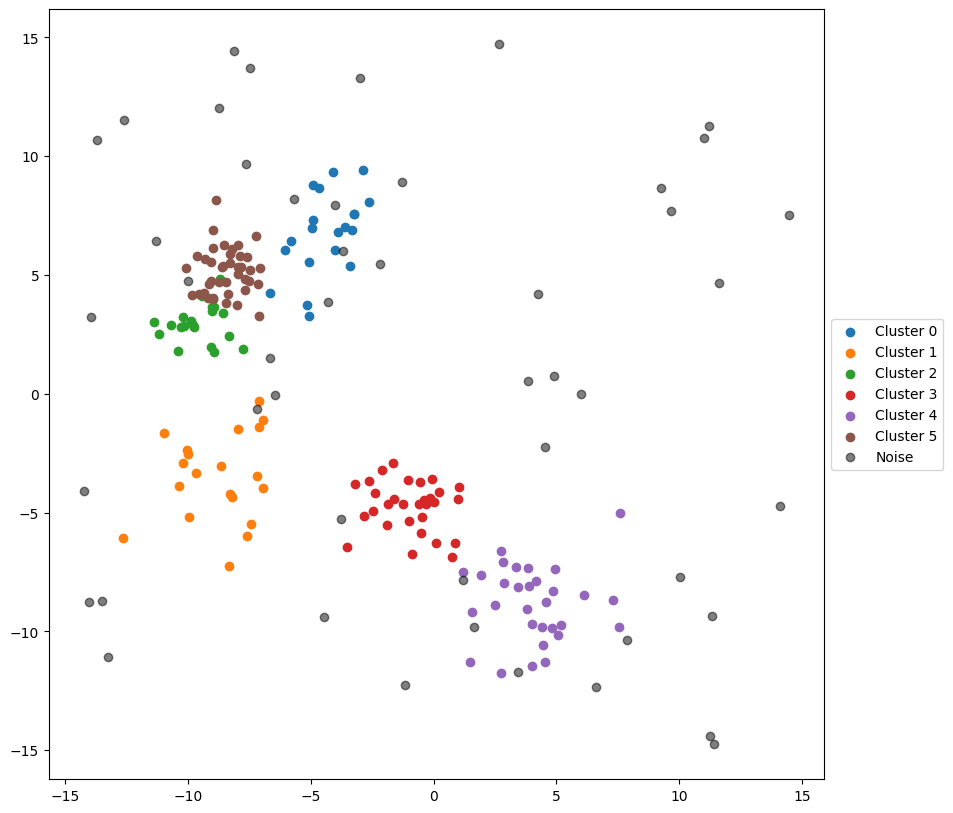
\includegraphics[width=0.9\linewidth]{Figures/dati_veri.png}
    \caption[example of data for clustering]{Data points are coloured according to their label, while noise is shown in grey.}
    \label{fig:data_true}
\end{figure}

\noindent Now let will try clustering with \gls{kmeans} using the right number of centroids, i.e. $6$. In \cref{fig:data_kmeans} we can see that the noise has created an additional cluster and two of the original clusters have merged into one. Although the result is quite satisfactory, it is not entirely clean.

\noindent Next, let is apply clustering with \gls{gmm} again using $6$ centroids. In \cref{fig:data_gmm} it can be seen that the weight of the cluster generated by the noise is very small. Furthermore, the covariance matrices allow the position of the centroids to be calculated more precisely, providing information on the nature of the clusters and creating a hierarchical structure. This is because, in reality, these are not real clusters, but normal distributions.

\noindent Finally, let clustering be applied with \gls{fcm} using $6$ centroids. In \cref{fig:data_fcm} we observe that the centroids are less affected by noise, making it possible to identify which data are potentially noisy or shared between several clusters.

\bigskip
We have observed that in the presence of noise, the algorithm \gls{fcm} can be very useful. However, the algorithm \gls{gmm}, although computationally onerous, also provides very valuable information about the nature of the data. In this thesis, we will use the \gls{fcm} algorithm to reduce the amount of information to be processed and the \gls{kmeans} algorithm for efficient initialisation of centroids.
